\vspace{1cm}
{\small%
\section{Theoreme der Feldtheorie}
\subsection{Elektromagnetische Energiebilanz}
\begin{itemize}
    \itemsep0pt
    \item \textbf{PEC} (\textit{perfectly electrically conducting}): \(E_{tan} = \vec{n} \times \vec{E} = 0\)
    \item \textbf{PMC} (\textit{perfectly magnetically conducting}): \(H_{tan} = \vec{n} \times \vec{H} = 0\)
    \item Komplexe Poynting-Vektor: \(\vec{S} = \dfrac{1}{2} \vec{E} \times \vec{H}^*\)
    \item Gesamte Verlustleistung: \(P_V = P_\kappa + P_\epsilon + P_\mu\)
    \item Zeitharmonische Vorgänge in einem abgeschlossenen, quellenfreien Gebiet:\\
        \[\oiint\limits_{A(V)}\vec{S}\cdot\mathrm{d}\vec{A} = - P_V + 2j\omega\,(\overline{W}_e - \overline{W}_m)\]
\end{itemize}
\subsection{Reziprozität}
\begin{itemize}
    \item \textbf{Allgemeine Form des Reziprozitätstheorems:}\\
        \begin{align*}
            &\iiint\limits_V\left(\vec{E}_1 \cdot \vec{J}_2 - \vec{H}_1 \cdot \vec{M}_2\right)\mathrm{d}v\\
            &= \iiint\limits_V\left(\vec{E}_2 \cdot \vec{J}_1 - \vec{H}_2 \cdot \vec{M}_1\right)\mathrm{d}v
        \end{align*}
\end{itemize}
\subsection{Elektromagnetische Potentiale}
\begin{itemize}
    \itemsep1pt
    \item Magnetische Vektorpotential \(\vec{B} = \nabla\times\vec{A}\)
    \item \textit{Helmholtz-Theorem} besagt, dass jede beliebige Vektorfeld im freien Raum geschrieben werden kann als:\\
        \(\vec{A} = \nabla\times\vec{C} + \nabla\xi\)
    \item Freiheitsgrad: \(\vec{B} = \nabla\times\vec{A} = \nabla\times\nabla\times\vec{C}\)
    \item Elektrische Skalarpotential $\varphi$:\\
        \(\vec{E} = -j\omega\vec{A} - \nabla\varphi\)
    \item \textbf{Vektorielle Helmholz-Gleichung:}\\
        \(\Delta\vec{A} + k^2\vec{A}  = -\mu\vec{J}\)
    \item \textbf{Skalare Helmholz-Gleichung:}\\
        \(\Delta\varphi + k^2\varphi = -\dfrac{\rho}{\epsilon}\)
    \item \textbf{Analog:} elektrische Vektorpotential $\vec{F}$ und skalare magnetische Potential $\psi$
        \begin{align*}
            \vec{D} &= -\nabla \times \vec{F}\\
            \vec{H} &= -j\omega\vec{F} - \nabla\psi
        \end{align*}
\end{itemize}
\subsection{Green'sche Funktionen}
\begin{itemize}
    \itemsep1pt
    \item Verhält sich wie ein \textit{Impulsantwort} der Feldlösung einer bestimmten Geometrie
    \item Poisson-Gleichung: \(\Delta G^\varphi(\vec{r}, \vec{r}^\prime) = -\dfrac{1}{\epsilon}\delta(\vec{r}, \vec{r}^\prime)\)
    \item Sind die Feldgrößen \textit{Skalare}, so ist die Green'sche Funktion ein \textit{Skalar}\\
        $\implies$ $\rho$ und $\varphi$ sind Skalare, also ist $G^\varphi$ ein Skalarfeld
    \item Sind die Feldgrößen \textit{Vektoren}, so ist die Green'sche Funktion eine \textit{Dyade}\\
        $\implies$ $\vec{J}$ und $\vec{A}$ sind Vektoren, also ist $\dyade{G}^A$ eine Dyade
        \begin{align*}
            \vec{A} &= \iiint\limits_V \dyade{G}^A(\vec{r},\vec{r}^\prime) \cdot \vec{J}(\vec{r}^\prime)\:\mathrm{d}v^\prime =\\
            &= \iiint\limits_V\
            \begin{pmatrix}\
                G^A_{xx}(\vec{r},\vec{r}^\prime) & G^A_{xy}(\cdot) & G^A_{xz}(\cdot)\\
                G^A_{yx}(\cdot) & G^A_{yy}(\cdot) & G^A_{yz}(\cdot)\\
                G^A_{zx}(\cdot) & G^A_{zy}(\cdot) & G^A_{zz}(\cdot)
            \end{pmatrix}\
            \begin{pmatrix}\
                J_x(\vec{r}^\prime)\\
                J_y(\vec{r}^\prime)\\
                J_z(\vec{r}^\prime)
            \end{pmatrix}\
            \mathrm{d}v^\prime
        \end{align*}
    \item Green'sche Funktionen \textbf{des freien Raumes:}\\
        \begin{align*}
            &G(\vec{r},\vec{r}^\prime) = \dfrac{\mathrm{e}^{-jk\:|\vec{r} - \vec{r}^\prime|}}{4\pi|\vec{r} - \vec{r}^\prime|},\\
            &\dyade{G}^A(\vec{r},\vec{r}^\prime) = \mu\dfrac{\mathrm{e}^{-jk\:|\vec{r} - \vec{r}^\prime|}}{4\pi|\vec{r} - \vec{r}^\prime|}\dyade{I},\\
            &\dyade{G}^F(\vec{r},\vec{r}^\prime) = \epsilon\dfrac{\mathrm{e}^{-jk\:|\vec{r} - \vec{r}^\prime|}}{4\pi|\vec{r} - \vec{r}^\prime|}\dyade{I}
        \end{align*}
    \item EM-Felder des freien Raumes, bei \textbf{Anregung mit elektrischen Strömen:}\\
        \begin{align*}
            &\dyade{G}^E_J(\vec{r},\vec{r}^\prime) = -j\omega\mu\left[\left(\dyade{I} + \dfrac{1}{k^2}\nabla\nabla\right) \dfrac{\mathrm{e}^{-jk\:|\vec{r} - \vec{r}^\prime|}}{4\pi|\vec{r} - \vec{r}^\prime|}\right]\\
            &\dyade{G}^H_J(\vec{r},\vec{r}^\prime) = \nabla\;\dfrac{\mathrm{e}^{-jk\:|\vec{r} - \vec{r}^\prime|}}{4\pi|\vec{r} - \vec{r}^\prime|} \times \dyade{I}\\
            &\vec{E} = -j\omega \left[\dyade{I} + \dfrac{1}{k^2}\nabla\nabla\right] \cdot \vec{A},\;\
            \vec{H} = \dfrac{1}{\mu} \nabla \times \vec{A}
        \end{align*}
    \item EM-Felder des freien Raumes, bei \textbf{Anregung mit magnetischen Strömen:}\\
        \begin{align*}
            &\dyade{G}^E_M(\vec{r},\vec{r}^\prime) = -\nabla\;\dfrac{\mathrm{e}^{-jk\:|\vec{r} - \vec{r}^\prime|}}{4\pi|\vec{r} - \vec{r}^\prime|} \times \dyade{I}\\
            &\dyade{G}^H_M(\vec{r},\vec{r}^\prime) = -j\omega\epsilon\left[\left(\dyade{I} + \dfrac{1}{k^2}\nabla\nabla\right) \dfrac{\mathrm{e}^{-jk\:|\vec{r} - \vec{r}^\prime|}}{4\pi|\vec{r} - \vec{r}^\prime|}\right]\\
            &\vec{E} = -\dfrac{1}{\epsilon} \nabla \times \vec{F},\;\
            \vec{H} = -j\omega \left[\dyade{I} + \dfrac{1}{k^2}\nabla\nabla\right] \cdot \vec{F}
        \end{align*}

\end{itemize}
\subsection{Spiegelungsprinzip}
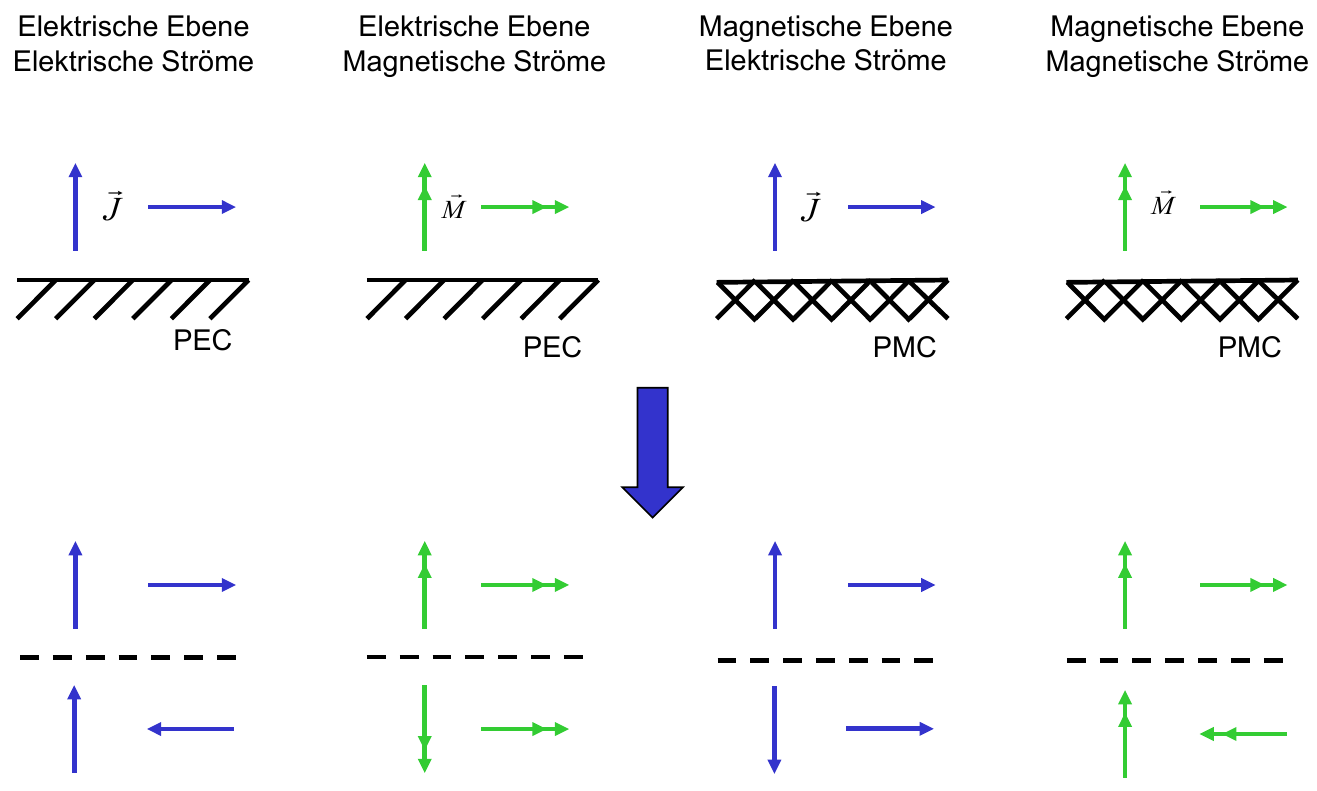
\includegraphics[width = 0.35\paperheight]{content/fuw/pictures/fuw_spiegelungsprinzip.png}
\subsection{Huygen'sches Prinzip}
\begin{itemize}
    \itemsep0pt
    \item Jede Wellenfront kann als Superposition von Elementarwellen dargestellt werden
    \item Math. Form des Huygens Prinzips:
        \begin{align*}
            \vec{E}(\vec{r}) = &\iiint\limits_{V_b}\
            \left[\
            \dyade{G}^E_J(\vec{r},\vec{r}^\prime)\cdot\vec{J}(\vec{r}^\prime) +\
            \dyade{G}^E_M(\vec{r},\vec{r}^\prime)\cdot\vec{M}(\vec{r}^\prime)\
            \right]\
            \mathrm{d}v^\prime\\
            + &\oiint\limits_{A(V_b)}\
            \left[\
            \dyade{G}^E_J(\vec{r},\vec{r}^\prime)\cdot\vec{J}_A(\vec{r}^\prime) +\
            \dyade{G}^E_M(\vec{r},\vec{r}^\prime)\cdot\vec{M}_A(\vec{r}^\prime)\
            \right]\
            \mathrm{d}a^\prime,\\
            &\vec{J}_A(\vec{r}^\prime) = \vec{n} \times \vec{H}(\vec{r}^\prime),\\
            &\vec{M}_A(\vec{r}^\prime) = -\vec{n} \times \vec{E}(\vec{r}^\prime)\\
        \end{align*}
    \item Nach Einführung von $\vec{J}_A$ und $\vec{M}_A$ ist das Volumen $V_a$ außerhalb des betrachteten Lösungsgebietes $V_b$ (formal mathematisch) \textit{feldfrei}
\end{itemize}
\subsection{Nahfeld und Fernfeld}
\begin{itemize}
    \itemsep0pt
    \item Fernfeld beginnt, wo die Wellenfronten näherungsweise eben sind und ein rein reeler Poynting-Vektor herrscht
    \item Math. Definition der Fernfeldgrenze mit Antennendurchmesser $D$:\\
        \(D_{FF} = \dfrac{2D}{\lambda}\)
    \item \textbf{Beobachtungskoordinaten im Fernfeld} (\(r\gg\lambda\)): Kugelkoordinaten
    \item Zwei unterschiedliche Fernfeld-Näherungen:\\
        \begin{itemize}
        \itemsep0pt
        \item Im Nenner (Amplitude): \(|\vec{r} - \vec{r}^\prime| \approx r\)
        \item Im Exponenten (Phase): \(|\vec{r} - \vec{r}^\prime| \approx r - \Delta r = r - \dfrac{\vec{r} \cdot \vec{r}^\prime}{r}\)
        \end{itemize}
    \item Es ergibt sich (Form analog zu Fourier):\\
            \begin{align*}
                &\vec{A}(\vec{r}) = \mu\dfrac{\mathrm{e}^{-jkr}}{4\pi r} \iiint\limits_V \vec{J}(\vec{r}^\prime) \mathrm{e}^{+jk\dfrac{\vec{r}^\prime \cdot \vec{r}}{r}} \:\mathrm{d}v^\prime\\
                &\vec{F}(\vec{r}) = \epsilon\dfrac{\mathrm{e}^{-jkr}}{4\pi r} \iiint\limits_V \vec{M}(\vec{r}^\prime) \mathrm{e}^{+jk\dfrac{\vec{r}^\prime \cdot \vec{r}}{r}} \:\mathrm{d}v^\prime
            \end{align*}
        \item Unter Vernachlässigung der aller räumlichen Abhängigkeiten außer $\dfrac{\mathrm{e}^{-jkr}}{r}$:\\
            \begin{align*}
                \nabla\times&\vec{A} \approx -jk\vec{e}_r\times\vec{A}\\
                \nabla\cdot&\vec{A} \approx -jk\vec{e}_r\cdot\vec{A}\\
                \implies&\
                \begin{cases}%
                    \vec{H}(\vec{r}) \approx -\dfrac{jk}{\mu}\vec{e}_r\times\vec{A}(\vec{r}),\\
                    \vec{E}(\vec{r}) \approx \dfrac{jk}{\epsilon}\vec{e}_r\times\vec{F}(\vec{r})
                \end{cases}
            \end{align*}
        \item Sphärische Feldkomponenten im Fernfeld; \textit{Elektrische Ströme}:
            \begin{align*}
                &H_{r1}=0, &E_{r1}=0,\\
                &H_{\vartheta1}=\dfrac{jk}{\mu}A_{\varphi}, &E_{\vartheta1}=-j\omega A_{\vartheta}=Z_F H_{\varphi1},\\
                &H_{\varphi1}=\dfrac{jk}{\mu}A_{\vartheta}, &E_{\varphi1}=-j\omega A_{\varphi}=-Z_F H_{\vartheta1}\\
            \end{align*}
        \item Sphärische Feldkomponenten im Fernfeld; \textit{Magnetische Ströme}:
            \begin{align*}
                &E_{r2}=0, &H_{r2}=0,\\
                &E_{\vartheta2}=-\dfrac{jk}{\epsilon}F_{\varphi}=Z_F H_{\varphi2}, &H_{\vartheta2}=-j\omega F_{\vartheta},\\
                &E_{\varphi2}=\dfrac{jk}{\epsilon}F_{\vartheta}=-Z_F H_{\vartheta2}, &E_{\varphi2}=-j\omega F_{\varphi}\\
            \end{align*}
        \item \(Z_F = \sqrt{\dfrac{\mu}{\epsilon}} = \dfrac{\omega\mu}{k}\)
\end{itemize}
}
